\documentclass[dvips,ruledheader]{abnt}
\usepackage[brazil]{babel} 					% linguagem portugues-Br
\usepackage[T1]{fontenc}
% \usepackage[latin1]{inputenc}
\usepackage[utf8]{inputenc} 				% para aceitar ascentos
\usepackage[pdftex]{graphicx}
% \usepackage[pdftex]{hyperref}
% \usepackage{hyperref}						% incluir links para web
\usepackage{abnt-alf}
\usepackage{latexsym}
\usepackage{psfrag}
\usepackage{epigraph}

% Glossário não utilizado
% \usepackage{makeglo}
% \renewcommand{\glossaryname}{Glossário}
% \makeglossary

\author{Álvaro Vilobaldo \emph{Rios}\\
Marcio \emph{Fernandes} Justino}

\begin{document}
\DeclareGraphicsRule{.eps.gz}{eps}{.eps.bb}{`gunzip -c #1}

%\include{encardenacao}
% \begin{figure}[topo]
%   \centering
%   \includegraphics[scale=0.3\textwidth]{figuras/}
%   \label{fig:comporte}
% \end{figure}


\titulo{Gestão de Obra\\
	Sistema de gestão de obras de engenharia\\
	Módulo I - Orçamento de Obra}

\instituicao{Rios Fernandes\par
Departamento de Desenvolvimento\par}

\local{São Bernardo do Campo -- SP}

\data{\today\par\LaTeX{}}

\capa
\folhaderosto

\tableofcontents

\part{Regras de Negócio}
\chapter{Obra}
Para construir ou reformar é preciso conhecer as etapas de uma obra, desde a contratação dos projetos de arquitetura até a limpeza do local.

Para a realização de uma obra são necessários alguns passos:

\begin{itemize}
	\item Contratação de escritório de arquitetura;
	\item Elaboração de ante-projeto de arquitetura;
	\item Elaboração dos projetos arquitetônicos;
	\item Aprovação do projeto legal na prefeitura;
	\item Contratação de escritório de projetos de estruturas e instalações;
	\item \emph{Elaboração do orçamento da obra};
	\item Elaboração do planejamento da obra; e
	\item Execução da obra.
\end{itemize}
\chapter{Projeto}
O projeto de orçamento deve possuir:

\begin{itemize}
	\item Um projeto pai\footnote{não obrigatório};
	\item Descrição do projeto;
	\item Cliente;
	\item Endereço (endereço físico do cliente);
	\item Orçamentos (orçamento de estimativa, de venda e de execução);
	\item Situação do projeto;
	\item Tipo de projeto (neste caso de orçamento);
	\item Fase do projeto; e
	\item \% de bonificação (lucro com o projeto).
\end{itemize}

O sistema deverá permitir a criação e alteração de um projeto. Para criar um novo projeto o usuário deve informar:
\begin{enumerate}
	\item Projeto pai (se existir);
	\item O cliente ao qual se destinará o projeto;
	\item O endereço do cliente onde o projeto será executado;
	\item A descrição do projeto;
	\item O tipo do projeto; e
	\item O percentual de bonificação (lucro com o projeto).
\end{enumerate}

Ao criar um projeto, o usuário pode utilizar um projeto como base para a formação do novo projeto, bastando localizar e informar o projeto modelo desejado.
\chapter{Orçamento}

Para construir ou reformar é preciso conhecer as etapas de uma obra, desde a contratação dos projetos de arquitetura até a limpeza do local. O orçamento é uma das etapas de elaboração de um projeto de construção ou reforma.

O orçamento de obra é a etapa onde se estabelecem os custos envolvidos na execução da obra, especificando as atividades necessárias para a aplicação do projeto (comumente nomeadas de \emph{serviços}), se aprofundando nos custos envolvidos para a execução de cada atividade, desde mão-de-obra e custo de material básico como cimento e areia, da utilização de recursos externos tais como equipamentos alugados e até mesmo mão-de-obra especializada, impostos envolvidos nas atividades, entre outros.

Um projeto pode apresentar diversos orçamentos, comumente criados como estimativas e ajustados até que se chegue ao orçamento de venda. O orçamento de venda é o orçamento de custos reais (que irá ser aprovado em uma concorrência).
O responsável pela elaboração do projeto cria um orçamento que inicialmente é nomeado de orçamento de ``estimativa''. Um orçamento de estimativa serve como base para a criação do orçamento de ``venda'', e também para manutenção de histórico do projeto. Todos os orçamentos de estimativa criados para o projeto são mantidos. Após a aprovação de um orçamento e o início de execução do projeto é necessário realizar o acompanhamento do projeto, que é feito a partir do orçamento de ``execução''. O orçamento de execução é originado com base no orçamento de venda, podendo sofrer ajustes e aditivos \textbf{não} previstos no orçamento de ``venda''. Já ajustes realizados com base no desejo são realizados no orçamento de ``venda'' e refletidos automaticamente para o orçamento de ``execução''.

Portanto, existem 3 tipos diferentes de orçamento:

\begin{description}
	\item[Estimativa] \hfill \\
	Esboços de orçamentos para o projeto (histórico do projeto);
	\item[Venda] \hfill \\
	Orçamento inicial com base no histórico; e
	\item[Execução] \hfill \\
	Orçamento guia de execução do projeto.
\end{description}

\section{Orçamento de Estimativa}

Este é o orçamento impreciso, estimado, quando um cliente solicita um orçamento prévio para realização de um determinado serviço, sendo esse somente uma estimativa pois, neste momento, não há um projeto definido, não se conhecem todas as atividades necessárias para sua execução - somente atividades básicas e não complexas.

Normalmente na fase de estimativa levam-se em conta projetos base \footnote{projetos criados para servir de base para outros, tendo pequenas diferenças em suas atividades} para facilitar a recuperação de atividades padronizadas, sendo modificadas somente algumas atividades em particular ao projeto que se estima ou a quantidade do serviço para o projeto em questão. Além de utilizar projetos base, mais comumente são utilizados padrões de projetos (apostilas que determinam os elementos base de um determinado projeto). Nesses casos, o usuário que define o projeto deverá seguir os padrões pré-estabelecidos para manter a conformidade de suas atividades.

\section{Orçamento de Venda}

Nesta fase, o orçamento é baseado em projeto bem definido pelo engenheiro, tendo suas atividades bem definidas, todos os custos diretos e indiretos de execução do projeto definidos.
A obtenção do custo real é baseada na estruturação dos serviços e suas composições (veremos o que são composições mais adiante), determinadas pela quantidade de cada item para a execução do serviço, como mostra a figura \ref{fig:composicao}.

\begin{figure}[htb]
	\centering
	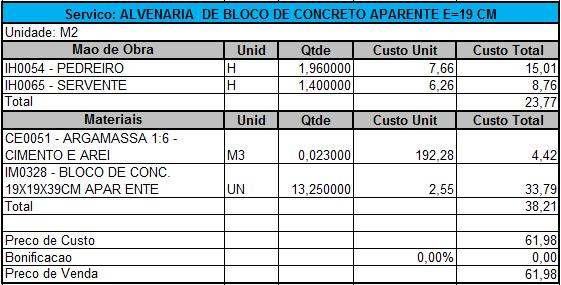
\includegraphics[width=0.9\textwidth]{figuras/composicao.jpg}
	\caption{Composição de um serviço}
	\label{fig:composicao}
\end{figure}

A definição do custo é a somatória de todos os recursos desprendidos na execução do projeto (custos diretos) e de todos os custos indiretos envolvidos.

Para o orçamento de venda, ainda constam os impostos e encargos sociais envolvidos e o lucro desejado com a execução do projeto (BDI).

Esse é o orçamento que é utilizado para \emph{vender o projeto} ao cliente. Após aprovado, o passo seguinte é acompanhar a execução do projeto com o orçamento de ``execução''.

\section{Orçamento de Execução}

Este orçamento, originado de um orçamento prévio de venda, recebe o realizado durante o projeto, provendo um comparativo futuro entre o que foi orçado e o que realmente foi executado. 

No orçamento de execução comumente surgem imprevistos que são registrados para reportar os custos reais do realizado e que não fora previsto pelo orçamento de venda. A figura \ref{fig:curva_abc} demonstra uma forma de comparativo entre ``previsto x realizado''.


\begin{figure}[htb]
	\centering
	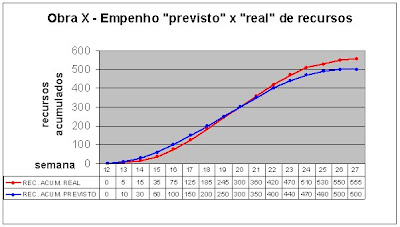
\includegraphics[width=0.9\textwidth]{figuras/curva_abc.jpg}
	\caption[Curva ABC]{Previsto x Realizado}
	\label{fig:curva_abc}
\end{figure}

Os serviços no orçamento devem ser agrupados como sendo de ``\textbf{custos diretos}'', de ``\textbf{custos indiretos}'' e ``\textbf{custos administrativos}''.
\chapter{Agrupamento}

Com o grande número de serviços prestados em um projeto, surge a necessidade de agrupar essas atividades em grupos de forma a facilitar a identificação com facilidade do grupo de atividades que devem ser executadas para uma determinada finalidade. Um grupo poderá conter outro grupo e/ou serviços ligados à ele.

Um bom exemplo seria a demonstração da imagem \ref{fig:agrupamento}. Nela podemos ver a subdivisão entre grupo, subgrupo e serviços. O grupo, neste caso, seria feito pelo ítem \emph{8 (Instalações Hidrosanitarias/Gas)}, o qual agrupa todos seus serviços ou outros grupos - no caso podem ser demonstrados pelos itens \emph{8.1 (Instalação hidráulica) e 8.2 (Instalações Prediais - Esgoto)}. Dentro dos subgrupos temos os serviços  distribuídos, a exemplo dos itens \emph{8.1.1; 8.2.2; ...; 8.1.12}.

\begin{figure}[htb]
\centering
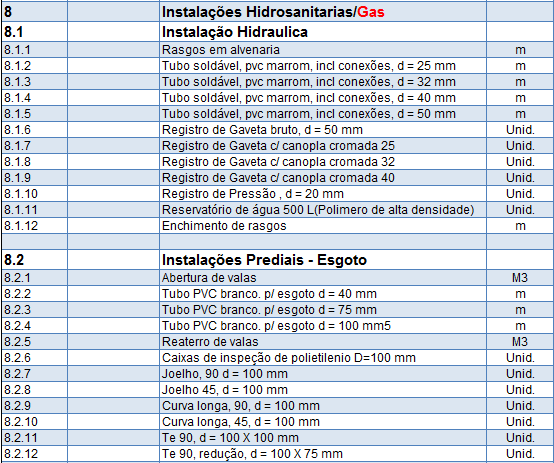
\includegraphics[width=0.7\textwidth]{figuras/agrupamento.png}
\caption{Demonstração de agrupamento de serviços}
\label{fig:agrupamento}
\end{figure}

Sendo assim, um agrupamento pode ter inúmeros outros agrupamentos que, ao final, remetem à um ou mais serviços.
\chapter{Serviço}

Serviço é uma atividade na qual a construtora está apta a realizar. Ex.:

\begin{itemize}
	\item Analise granulometrica sem sedimentacao;
	\item Ensaio para determinacao do Indice Suporte California (CBR) - 3 pontos - obtido com energia Proctor Intermediario, atraves de, no minimo, 5 corpos de prova, conforme recomendacao da NBR9895, NBR6457, NBR7182; ou
	\item Alvenaria de tijolo macico (7x10x20)cm, com argamassa de cimento e saibro no traco 1:6, em paredes com vaos ou arestas, de meia vez (0,10m), ate 3m de altura, e medida pela area real.
\end{itemize}

\emph{Inclusive alguns serviços como o uso de engenheiros da contrutora como se fosse uma consultoria.}

\section{Unidade de medição}

Todo seviço possui uma unidade de medição (quilometro, horas, metros etc), justamente para determinar o preço do serviço. Ex., a ``Alvenaria de tijolo macico'', mostrada acima é cobrada por metro quadrado (m2), ou seja, para cada m2 é utilizado todos os recursos alocados (Composição) nas suas devidas proporções já pré-determinadas e tem um custo já estipulado.

\section{Custo}

Cada unidade do serviço possui um custo. Esse custo é estipulado com base nos recursos utilizados, assim se para fazer uma um m2 de parede (serviço) é preciso utilizar um saco de cimento e dois de area para fazer uma parede de X metros serão necessários X sacos de cimento e 2X de areia.
\chapter{Composição}

Composição é o nome que se dá à junção de recursos desprendidos em uma determinada atividade, é o vinculo entre serviço, recurso e outros serviços alocados para o mesmo.

Por exemplo, uma atividade de \emph{Alv. Bl. Concreto 9x19x39 vedação} teria como composição os seguintes items:

\begin{table}[h]
	\centering
	\begin{tabular}{|l|l|c|r|}
	\hline
	Código&			Descrição&						Unidade&		Valor 	\\ \hline
	3.36.020&		bloco concreto 9x19x39&			pç&				13,13	\\ \hline
	3.05.300&		Arg. Serrana F11 saco 40kg&		kg&				17,78	\\ \hline
	2.10.020&		Pedreiro&						h&				 1,00	\\ \hline
	2.10.050&		Servente&						h&				 1,00	\\ \hline
	\end{tabular}
	\caption{Composição de atividade \emph{Alv. Bl. Concreto 9x19x39 vedação}. Cada item é considerado um recurso}
	\label{tab:composicao}
\end{table}

Para realizar determinado serviço serão necessários usar recursos estipulados e outros serviços. Essa listagem do ``que'' tem que ser feito para fazer um serviço se da o nome de composição. Ex., para fazer o recurso ``Cobertura em telhas onduladas, sem amianto, com espessura de 4mm, fixadas por pregos, inclusive vedacao, exclusive o madeiramento, Vogatex ou similar. Fornecimento e colocacao.'' será necessário usar os seguintes recursos:

\begin{itemize}
	\item 3\% incidente sobre mao de obra direta com Encargos Sociais para cobrir despesas de EPI e ferramentas;
	\item Conjunto de vedacao para telha ondulada (arruela galvanizada com borracha)
	\item Prego com cabeca, de (18x30);
	\item Telha ondulada sem amianto, com espessura de 4mm, medindo: (2,44x0,50)m, Vogatex ou similar;
	\item Carpinteiro - forma de concreto;
	\item Servente Tributos sobre o faturamento (7.56\%);
\end{itemize}

E o serviço de por exemplo, fixar colunas.
\chapter{Recurso}

Recurso é tudo que representa unidade e que compõe as atividades (serviços) de um projeto. 

\section{Tipo de Recurso}

O recurso é subdividido em: 

\begin{itemize}
	\item Materiais;
	\item Mão de Obra;
	\item Equipamento; e
	\item Encargos.
\end{itemize}

\section{Unidade de Recurso}

Os recursos são medidos por unidades:

\begin{itemize}
	\item Kilograma (kg);
	\item Litro (l);
	\item Hora/Homem (h);
	\item Metro cúbico (M3);
	\item Metro quadrado (M2); e
	\item Outros.
\end{itemize}

O custo do recurso é dado por unidade, como demonstra a tabela \ref{tab:composicao}. Os valores são representados para uma única unidade de cada recurso, sendo que uma atividade poderá consumir \emph{n} quantidades de recursos.

Um exemplo para a atividade \emph{Alv. Bl. Concreto 9x19x39} para construção de uma parede de 8m x 3m (24 m2). Assim, de acordo com a tabela de composição do serviço \ref{tab:composicao}, o serviço \emph{Alv. Bl. Concreto 9x19x39 vedação} tem um custo de 39,91 por m2. Para a execução da parede utilizando a atividade acima, seriam necessárias 24 unidades, totalizando seu custo em 957,84.
\chapter{Custos}

Os custos envolvidos no orçamento variam conforme a região onde o projeto é executado. Sendo assim, o sistema deverá permitir que um orçamento seja vinculado à uma região. Além do projeto, os serviços presentes em um orçamento possuem recursos que são originados de fornecedores, sejam materiais, sejam equipamentos ou mão de obra, assim, os preços também variam por fornecedor, e claro, por região.

Outro custo que pode variar com a região são os tributos.

A região deverá ser estabelecida através da ligação entre cidades.

\section{Região}

O sistema deverá permitir:

\begin{itemize}
	\item Incluir/Alterar/Remover uma região;
	\item Associar/Desassociar cidades a uma região; e
	\item Associar/Desassociar tributos a uma região.
\end{itemize}

A região deverá possuir:

\begin{itemize}
	\item Nome.
\end{itemize}

\section{Cliente}

O sistema deverá permitir:

\begin{itemize}
	\item Incluir/Alterar/Remover um cliente;
	\item Associar/Desassociar endereços a um cliente; e
	\item Associar/Desassociar um cliente/endereço a um projeto.
\end{itemize}

O cliente deverá possuir:

\begin{itemize}
	\item Nome; e
	\item Endereços.
\end{itemize}

\section{Endereço}

O sistema deverá permitir:

\begin{itemize}
	\item Incluir/Alterar/Remover um endereço para um cliente; e
	\item Incluir/Alterar/Remover um endereço para um fornecedor.
\end{itemize}

O endereço deverá possuir:

\begin{itemize}
	\item Tipo de logradouro (Rua, Avenida, etc.);
	\item Cidade;
	\item CEP;
	\item Logradouro;
	\item Complemento; e
	\item Numero.
\end{itemize}

\section{Fornecedor}

O sistema deverá permitir:

\begin{itemize}
	\item Incluir/Alterar/Remover um fornecedor;
	\item Incluir/Alterar/Remover endereços de um fornecedor; e
	\item Incluir/Alterar/Remover preços de insumos de um fornecedor.
\end{itemize}

Um fornecedor deverá possuir:

\begin{itemize}
	\item Nome;
	\item CNPJ;
	\item Inscrição Estadual; e
	\item Tipo de fornecedor.
\end{itemize}

\section{Tipo de Fornecedor}

O sistema deverá permitir:

\begin{itemize}
	\item Incluir/Alterar/Remover um tipo de fornecedor; e
	\item Alterar tipo de fornecedor de um fornecedor.
\end{itemize}

O tipo de fornecedor deverá possuir:

\begin{itemize}
	\item Descrição.
\end{itemize}

\section{Cidade}

O sistema deverá permitir:

\begin{itemize}
	\item Incluir/Alterar/Remover uma cidade em um estado;
	\item Associar/Desassociar uma cidade a uma região; e
	\item Associar/Desassociar uma cidade de uma região.
\end{itemize}

Uma cidade deverá possuir:

\begin{itemize}
	\item Estado;
	\item Região; e
	\item Nome da cidade.
	\item Incluir/Alterar/Remover um endereço para um fornecedor.
\end{itemize}

\section{Estado}

O sistema deverá permitir:

\begin{itemize}
	\item Incluir/Alterar/Remover um estado em um país;
	\item Associar/Desassociar cidades a um estado; e
	\item Associar/Desassociar o estado a um país.
\end{itemize}

O estado deverá possuir:

\begin{itemize}
	\item País; e
	\item Nome.
\end{itemize}

\section{País}

O país deverá permitir:

\begin{itemize}
	\item Incluir/Alterar/Remover um país; e
	\item Associar/Desassociar estados a um país.
\end{itemize}

O país deverá possuir:

\begin{itemize}
	\item Nome.
\end{itemize}
\chapter{Taxas}

********** verificar este item depois **********
As taxas, tributos e encargos sociais são normalmente ministrados como recursos nos serviços.
\chapter{Região}

Todos os custos relacionados ao projeto devem ser identificados por região, tendo em vista que os preços de mão de obra, materiais e equipamentos variam de acordo com a região em que o projeto está sendo executado.

Um exemplo disso é a comparação de um projeto realizado em uma região de São Paulo (Interior) e outro que é realizado em uma outra região de São Paulo (Litoral). Nesses casos há uma diferenciação de preço de materiais, equipamentos e principalmente de mão de obra.

Uma região é composta por um determinado número de cidades sendo que uma cidade não pode estar em mais de uma região ao mesmo tempo.

\part{Requisitos Funcionais}
\chapter{Projeto}
O projeto de orçamento deve possuir:

\begin{itemize}
	\item Um projeto pai\footnote{não obrigatório};
	\item Descrição do projeto;
	\item Cliente;
	\item Endereço (endereço físico do cliente);
	\item Orçamentos (orçamento de estimativa, de venda e de execução);
	\item Situação do projeto;
	\item Tipo de projeto (neste caso de orçamento);
	\item Fase do projeto; e
	\item \% de bonificação (lucro com o projeto).
\end{itemize}

O sistema deverá permitir a criação e alteração de um projeto. Para criar um novo projeto o usuário deve informar:
\begin{enumerate}
	\item Projeto pai (se existir);
	\item O cliente ao qual se destinará o projeto;
	\item O endereço do cliente onde o projeto será executado;
	\item A descrição do projeto;
	\item O tipo do projeto; e
	\item O percentual de bonificação (lucro com o projeto).
\end{enumerate}

Ao criar um projeto, o usuário pode utilizar um projeto como base para a formação do novo projeto, bastando localizar e informar o projeto modelo desejado.
\chapter{Orçamento}

Para construir ou reformar é preciso conhecer as etapas de uma obra, desde a contratação dos projetos de arquitetura até a limpeza do local. O orçamento é uma das etapas de elaboração de um projeto de construção ou reforma.

O orçamento de obra é a etapa onde se estabelecem os custos envolvidos na execução da obra, especificando as atividades necessárias para a aplicação do projeto (comumente nomeadas de \emph{serviços}), se aprofundando nos custos envolvidos para a execução de cada atividade, desde mão-de-obra e custo de material básico como cimento e areia, da utilização de recursos externos tais como equipamentos alugados e até mesmo mão-de-obra especializada, impostos envolvidos nas atividades, entre outros.

Um projeto pode apresentar diversos orçamentos, comumente criados como estimativas e ajustados até que se chegue ao orçamento de venda. O orçamento de venda é o orçamento de custos reais (que irá ser aprovado em uma concorrência).
O responsável pela elaboração do projeto cria um orçamento que inicialmente é nomeado de orçamento de ``estimativa''. Um orçamento de estimativa serve como base para a criação do orçamento de ``venda'', e também para manutenção de histórico do projeto. Todos os orçamentos de estimativa criados para o projeto são mantidos. Após a aprovação de um orçamento e o início de execução do projeto é necessário realizar o acompanhamento do projeto, que é feito a partir do orçamento de ``execução''. O orçamento de execução é originado com base no orçamento de venda, podendo sofrer ajustes e aditivos \textbf{não} previstos no orçamento de ``venda''. Já ajustes realizados com base no desejo são realizados no orçamento de ``venda'' e refletidos automaticamente para o orçamento de ``execução''.

Portanto, existem 3 tipos diferentes de orçamento:

\begin{description}
	\item[Estimativa] \hfill \\
	Esboços de orçamentos para o projeto (histórico do projeto);
	\item[Venda] \hfill \\
	Orçamento inicial com base no histórico; e
	\item[Execução] \hfill \\
	Orçamento guia de execução do projeto.
\end{description}

\section{Orçamento de Estimativa}

Este é o orçamento impreciso, estimado, quando um cliente solicita um orçamento prévio para realização de um determinado serviço, sendo esse somente uma estimativa pois, neste momento, não há um projeto definido, não se conhecem todas as atividades necessárias para sua execução - somente atividades básicas e não complexas.

Normalmente na fase de estimativa levam-se em conta projetos base \footnote{projetos criados para servir de base para outros, tendo pequenas diferenças em suas atividades} para facilitar a recuperação de atividades padronizadas, sendo modificadas somente algumas atividades em particular ao projeto que se estima ou a quantidade do serviço para o projeto em questão. Além de utilizar projetos base, mais comumente são utilizados padrões de projetos (apostilas que determinam os elementos base de um determinado projeto). Nesses casos, o usuário que define o projeto deverá seguir os padrões pré-estabelecidos para manter a conformidade de suas atividades.

\section{Orçamento de Venda}

Nesta fase, o orçamento é baseado em projeto bem definido pelo engenheiro, tendo suas atividades bem definidas, todos os custos diretos e indiretos de execução do projeto definidos.
A obtenção do custo real é baseada na estruturação dos serviços e suas composições (veremos o que são composições mais adiante), determinadas pela quantidade de cada item para a execução do serviço, como mostra a figura \ref{fig:composicao}.

\begin{figure}[htb]
	\centering
	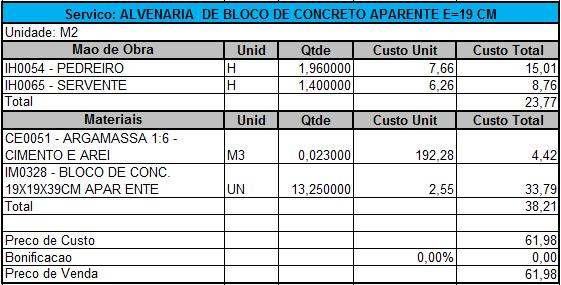
\includegraphics[width=0.9\textwidth]{figuras/composicao.jpg}
	\caption{Composição de um serviço}
	\label{fig:composicao}
\end{figure}

A definição do custo é a somatória de todos os recursos desprendidos na execução do projeto (custos diretos) e de todos os custos indiretos envolvidos.

Para o orçamento de venda, ainda constam os impostos e encargos sociais envolvidos e o lucro desejado com a execução do projeto (BDI).

Esse é o orçamento que é utilizado para \emph{vender o projeto} ao cliente. Após aprovado, o passo seguinte é acompanhar a execução do projeto com o orçamento de ``execução''.

\section{Orçamento de Execução}

Este orçamento, originado de um orçamento prévio de venda, recebe o realizado durante o projeto, provendo um comparativo futuro entre o que foi orçado e o que realmente foi executado. 

No orçamento de execução comumente surgem imprevistos que são registrados para reportar os custos reais do realizado e que não fora previsto pelo orçamento de venda. A figura \ref{fig:curva_abc} demonstra uma forma de comparativo entre ``previsto x realizado''.


\begin{figure}[htb]
	\centering
	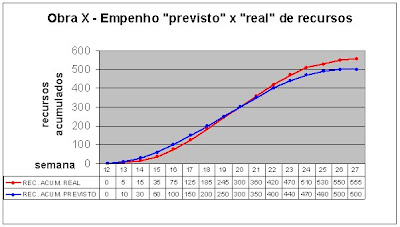
\includegraphics[width=0.9\textwidth]{figuras/curva_abc.jpg}
	\caption[Curva ABC]{Previsto x Realizado}
	\label{fig:curva_abc}
\end{figure}

Os serviços no orçamento devem ser agrupados como sendo de ``\textbf{custos diretos}'', de ``\textbf{custos indiretos}'' e ``\textbf{custos administrativos}''.
\chapter{Serviço}

Serviço é uma atividade na qual a construtora está apta a realizar. Ex.:

\begin{itemize}
	\item Analise granulometrica sem sedimentacao;
	\item Ensaio para determinacao do Indice Suporte California (CBR) - 3 pontos - obtido com energia Proctor Intermediario, atraves de, no minimo, 5 corpos de prova, conforme recomendacao da NBR9895, NBR6457, NBR7182; ou
	\item Alvenaria de tijolo macico (7x10x20)cm, com argamassa de cimento e saibro no traco 1:6, em paredes com vaos ou arestas, de meia vez (0,10m), ate 3m de altura, e medida pela area real.
\end{itemize}

\emph{Inclusive alguns serviços como o uso de engenheiros da contrutora como se fosse uma consultoria.}

\section{Unidade de medição}

Todo seviço possui uma unidade de medição (quilometro, horas, metros etc), justamente para determinar o preço do serviço. Ex., a ``Alvenaria de tijolo macico'', mostrada acima é cobrada por metro quadrado (m2), ou seja, para cada m2 é utilizado todos os recursos alocados (Composição) nas suas devidas proporções já pré-determinadas e tem um custo já estipulado.

\section{Custo}

Cada unidade do serviço possui um custo. Esse custo é estipulado com base nos recursos utilizados, assim se para fazer uma um m2 de parede (serviço) é preciso utilizar um saco de cimento e dois de area para fazer uma parede de X metros serão necessários X sacos de cimento e 2X de areia.

\part{Features}
\chapter{Recursos Futuros}

\section{Fornecedor}

Cadastrar fornecedor e preços de recursos para o fornecedor. Provavelmente disponibilizar um webservice para que o próprio fornecedor atualize seus valores.

\section{Preço}

Curva ABC de preço médio por região.

Gerar preço médio, para região, de acordo com o preço dos fornecedores da região.

Gráfico da curva ABC.

\section{Região}

Identificação automática de região através de cerca de região por google maps, localizando pelo endereço do cliente.

Cadastrar cidades. Vincular cidades à região.

\section{Orçamento}

Orçamento poderá ser feito pela média da região, por fornecedor(res) mais barato(s) ou de fornecedores específicos.

\section{Compras}

Vínculo do orçamento aprovado (Orçamento Inicial) com o módulo de compras, com situação de pré-compra.

Análise de preço de fornecedores para aquisição de recursos - alteração de situação de pré-compra para solicitação de autorização de compra. O operador de compras poderá alterar o fornecedor da forma que melhor lhe convir.

\section{Acompanhamento de Obra}

Estilo project do gerenciamento da obra em execução.

Confronto do orçamento de execução com o orçamento inicial (aprovado pelo cliente).

Diário de obra.





% \bibliography{bb}
% \bibliographystyle{abnt-alf}
\end{document}